\chapter{基于智能手机的两层多策略行为识别框架}

\par 在人体行为识别的基础之上应用极为广泛的应用,它们可以给现代人的娱乐生活、医疗健康等诸多方面带来极大的便利与帮助。而对于此类应用,准确地感知和识别用户姿势或行为是其中最为关键的核心任务。为了感知和识别用户行为,首先需要比较方便并且具有较少用户侵入性地采集有关人体的行为数据,其次需要设备具有能力传输或者处理数据,进一步判断和识别用户行为。近些年随着智能手机的不断发展,仅仅通过智能手机这一个设备已经具备了上述条件。首先智能手机内部集成有多种传感器,可以很好地采集用户的运动信息,其次智能手机的应用越来越广泛,其与现代人的关系也愈加密切,因此它可以方便且无侵入性的长期监测用户的运动信息。最后智能手机的存储和计算能力不断增强,现在已经完全可以应对提取特征,运行分类算法等复杂计算,因此可以很好地完成识别任务,且避免了传感器数据通信的麻烦。
\par 基于智能手机进行行为识别,不仅应用方便灵活,而且研究者也通过实验表明内置的多种类型传感器可以有效提高识别准确率。未来随着智能手机的不断进步和发展,基于智能手机的行为识别具有良好的应用前景。但是,智能手机在使用方便灵活的同时也存在着其他的问题。由于它的不固定,其位置和方向的变化会对内置传感器所采集的运动数据产生很大干扰,对最终的识别结果影响较大。因此我们需要提出新的解决方法降低这方面的影响。
\par 为解决上述问题,本章提出一种基于智能手机的两层多策略行为识别方案框架,其流程框图如图所示,框架主要包括数据获取,分组算法和多策略分类三部分。首先多个传感器以固定的采样率采集关于人体的行为数据信息。同时为了可以实现实时地行为识别,本文采用带有重叠的滑动窗口机制对智能手机所采集的传感器数据分割为固定窗口时间长度的数据段,然后对于每一段数据提取若干行为特征组成特征向量。基于这一特征向量,根据不同的行为分类问题通过信息增益排序的方式选择最佳特征子集用于训练相应的分类器并使用该分类器完成最终的分类任务。在本文的框架中,行为分类由两层组成,首先在第一层中为分组模型,即根据行为之间的相似程度被分为若干组。然后在第二层中根据不同组的行为的不同特点使用不同策略和相应的最佳分类器进行最后的分类。
\begin{figure}[ht]
\centering
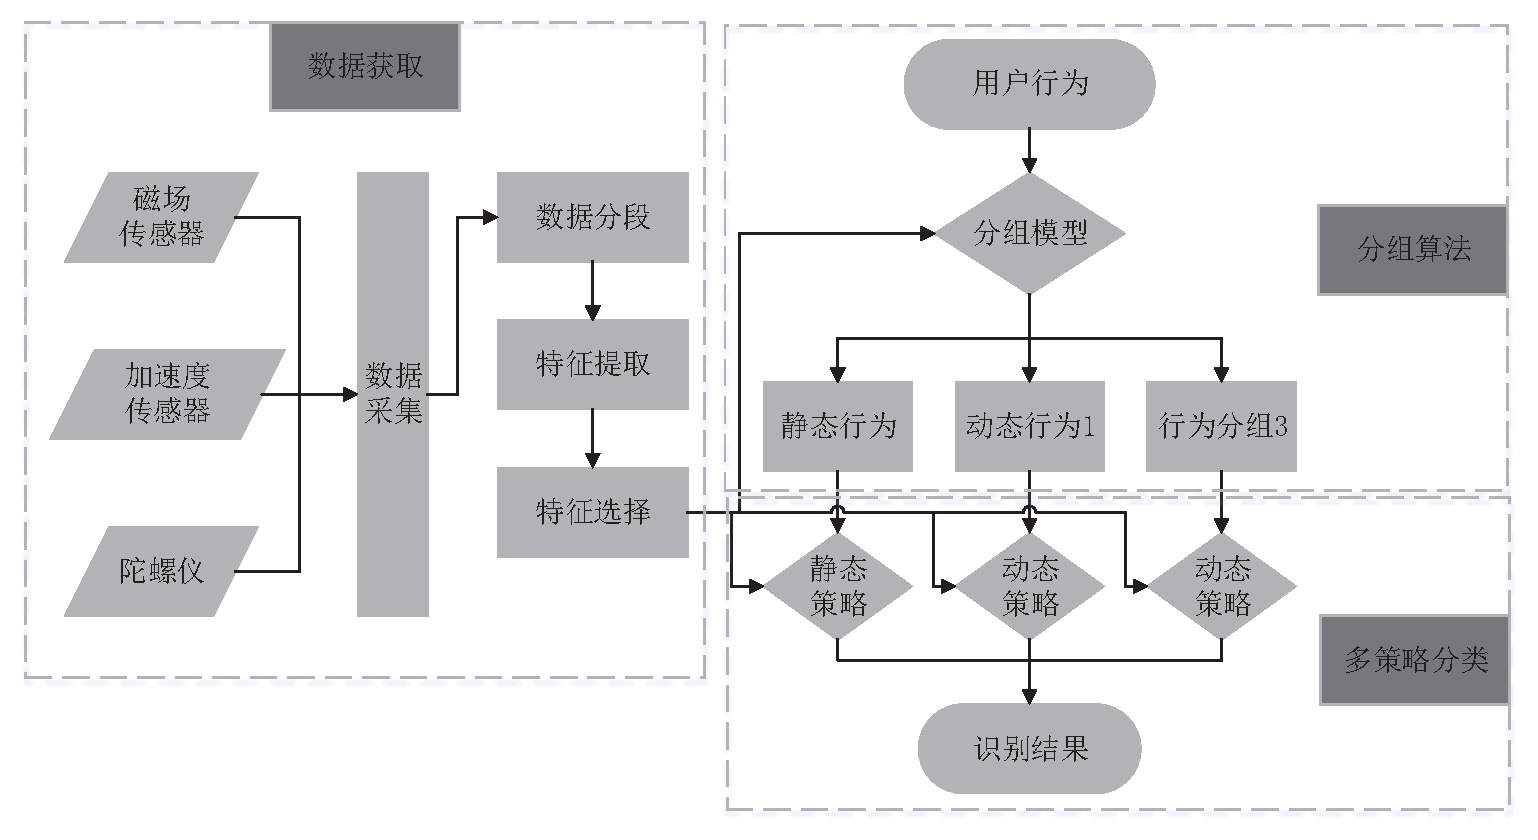
\includegraphics[width=15cm]{framework.eps}
\caption{两层多策略的行为识别框架流程图}
\end{figure}

\section{数据获取与处理}
\subsection{数据采集}
在本文的框架中,数据集主要来自几乎所有智能手机内部都有集成的三类传感器,包括加速度传感器,陀螺仪和磁场传感器。每个传感器都以采样率 采集数据并且采用长度为 以及重叠为50\%的滑动窗口对数据进行分割,最后每一段数据生成一个四维的信号向量$(x, y, z, magnitude)$, 基于数据向量就可以进行提取特征。 其中:
\begin{equation}
	magnitude = \sqrt{x^2+y^2+z^2}
\end{equation}


\subsection{特征提取}
本文中所使用的全部特征列举在表格1中, 主要包括时域的特征、频域的特征和关于自相关函数的特征。
\begin{table}[!htbp]
    \centering
    \caption{本文用到的特征列表}\label{tab:aStrangeTable}
    \begin{tabular}{cll}
    \toprule
    类别 & 特征 & 符号\\
    \midrule
    \multirow{4}*{时域特征}
    & 信号均值 & $\mu(\textbf{x})$\\
    & 信号方差 & $\sigma^2(\textbf{x})$\\
    & 窗口差值 & $\mu T$ \\
    & 窗口偏差 & $\mu D$ \\
    \bottomrule
    \end{tabular}
    \end{table}

下面以向量$\textbf{x}$为例说明上述系列特征的细节,其中向量$\textbf{x}$的长度为$N$。
\begin{itemize}
	\item 时域特征
\end{itemize}
\par 时域特征包括均值和方差等,计算简单并且可以有助于区分静止和动态行为,其中窗口差值和窗口偏差计算公式如下:
\begin{equation}
	\mu T = \sum_{i=2}^{M}(|\mu_i - \mu_{i-1}|)
\end{equation}
\begin{equation}
	\mu D = \sum_{i=1}^{M}(|\mu_i - \mu|)
\end{equation}
其中, 窗口长度为$N$的向量$\textbf{x}$被分割为$M$段,$\mu_i$表示第$i$段数据的均值,$\mu$表示向量$\textbf{x}$的均值。
\begin{itemize}
	\item 频域特征
\end{itemize}
\par 本文中频域信号主要是通过快速傅里叶变换(Fast Fourier Transform, FFT)算法计算得到得。在频域中,我们重点关注最大频域分量以及频域的能量值。频域特征与位置信息相关性较小,可以用来区分动态行为,而受到来自位置变化的影响较小。
\begin{itemize}
	\item 自相关函数特征
\end{itemize}
\par 信号的自相关函数可以通过公式计算得到。其中加速度数据和陀螺仪数据信号的自相关函数的图像分别如图2所示。
\begin{equation}
	R_x[i]=\frac{1}{N}\sum_{j=i}^{N-1} x[j]x[j-i]\qquad  i=0, 1, \cdots, N-1
\end{equation}
\begin{figure}[!htb]
    \centering
    \subfigure[The ACFs of Accelerometer]{
    \label{Fig.sub.1}
    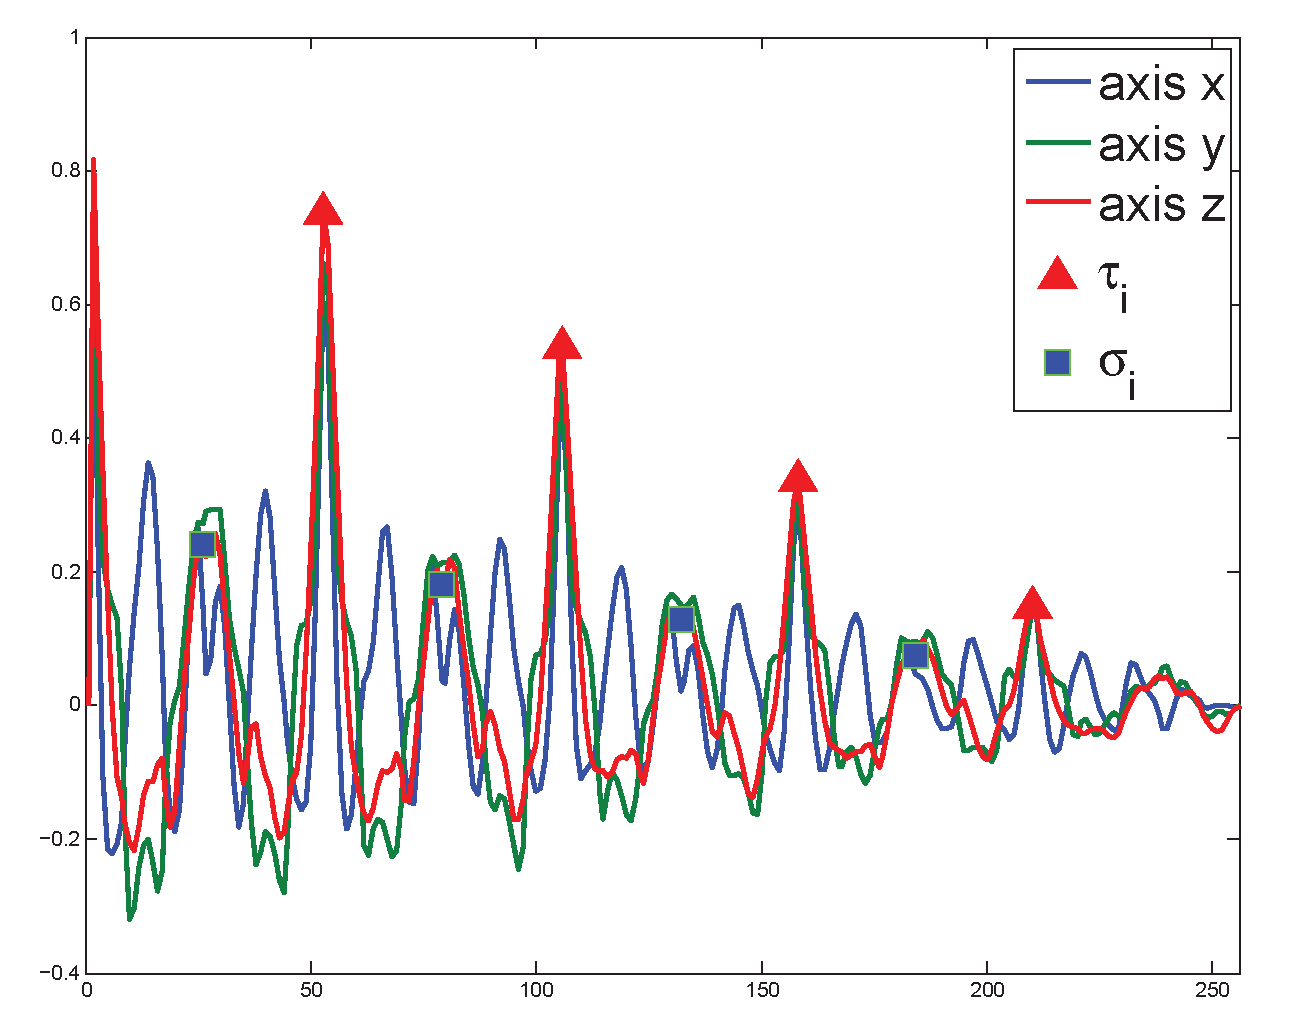
\includegraphics[width=0.45\textwidth]{acc_three_dimen5.eps}}
    \subfigure[The ACFs of Gyroscope]{
    \label{Fig.sub.2}
    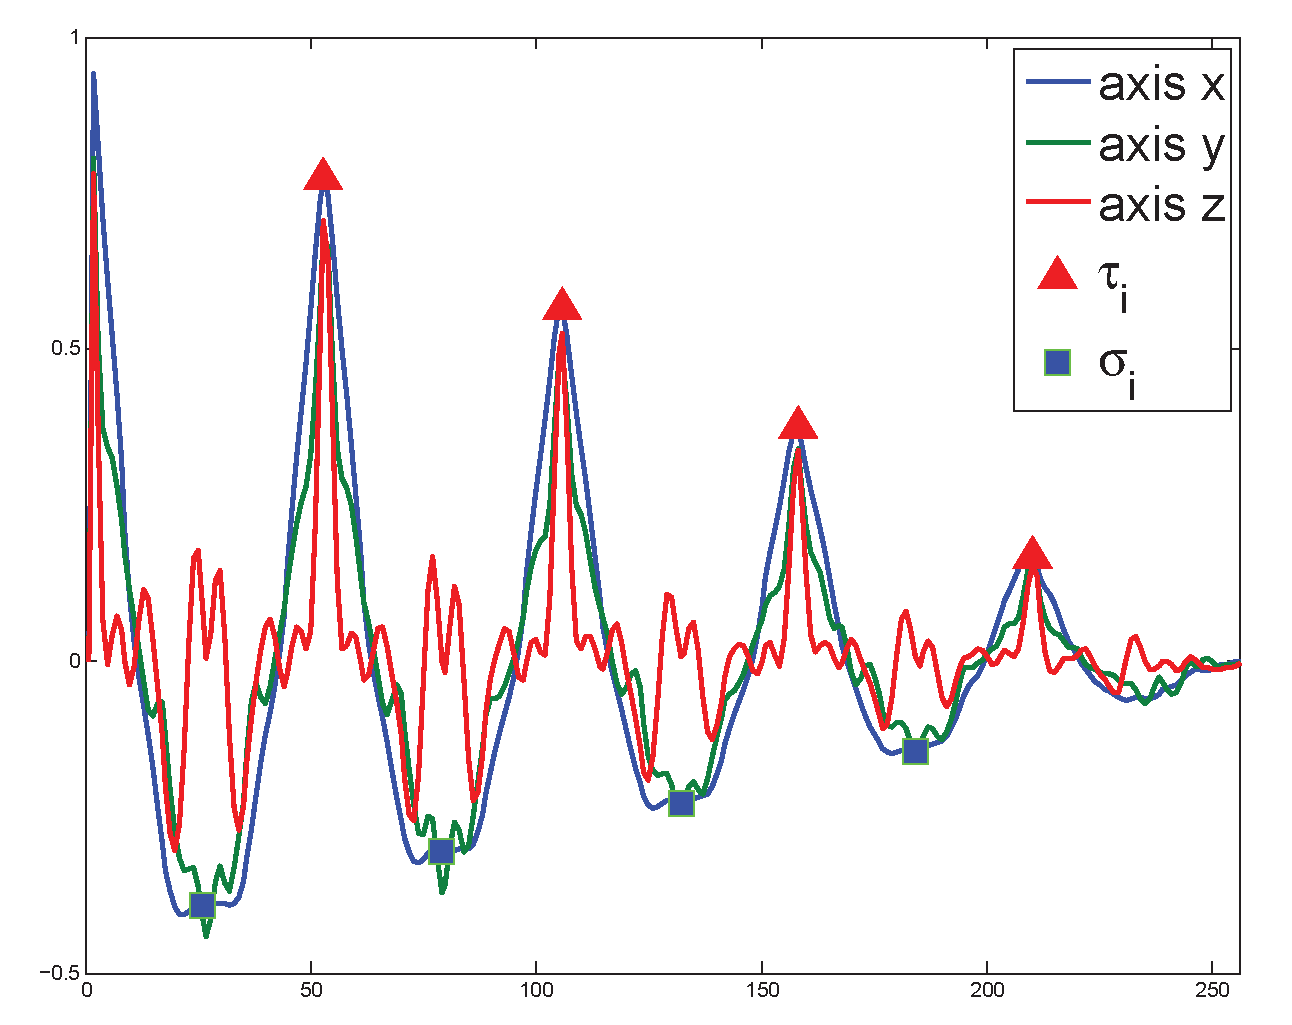
\includegraphics[width=0.45\textwidth]{gyro_three_dimen5.eps}}
    \caption{The ACFs of three-dimensional signals}
    \label{Fig.lable}
\end{figure}

\par 如图2所示,传感器数据三维信号的自相关函数在同一点取得极值,我们记为 $\sigma_i$,表示自相关函数的第$i$个极值。由于加速度传感器和陀螺仪是集成在同一部智能手机当中,因此他们所采取的数据计算相关函数极值的位置也相同。如果将它们各自的三维自相关函数加在一起就可以使得极值更加明显,不易被噪声混淆。另外使用自相关函数的和而非使用三轴向的传感器数据各自提取特征可以有效减少因为方向变化带来的影响。因此,在本文中关于自相关函数的特征都是使用自相关函数的和,即$R = R_x + R_y + R_z$,而不是每一维数据的自相关函数。
\par 使用自相函数的和计算以下特征,其中本文中使用前m个极值,计算公式如下:
\begin{equation}
    R_M = \frac {1}{m}\sum_{i=1}^m R[\tau_i]
\end{equation}
\begin{equation}
    P = \frac{1}{m}\sum_{i=1}^m {(\tau_i-\tau_{i-1})}
\end{equation}
\begin{equation}
    Diff = \frac{1}{m}\sum_{i=1}^m \sum_{j=\tau_i-3}^{j=\tau_i+3} {|R[j]-R[j-1]|} 
\end{equation}
\par 关于自相关函数的其他特征都与相邻极值中点$\sigma_i$ 处的函数值有关。在本文中,自相关函数相邻极值中点$\sigma_i$ 附近的一系列函数值被抽象为一个向量,比如 $\textbf{r}=\frac {1}{m} \sum_{i=1}^m\{R[j]\}, j=\sigma_i-3, \sigma_i-2,\cdots,\sigma_i+3$。这一向量的最大值、最小值和平均值被作为本方案中最后三个特征,分别表示为$Mid_M$, $Mid_m$, $Mid_\mu$。关于自相关函数的特征具有方向独立性的特点,因此可以有效区分动态行为而受到来自方向变化的影响较小。
\par 在本方案中使用的三个传感器传感器,时域和频域特征从四维数据中提起包括三轴方向和模值,即$d=\sqrt{x^2+y^2+z^2}$,共组成60维特征向量。而自相关函数的特征则是提取自加速度传感器和陀螺仪的三轴方向的自相关数之和,即组成12维自相关函数特征集。因此最终的特征向量共有72维,然后对于不同的分类任务,分别计算这些特征的信息增益并排序,最终为不同的分类问题选择最佳特征集。通过为不同分类任务选择维数较小的特征数量,不但可以有效减少特征计算的复杂度,而且可以有效利用不同特征在不同分类问题中的优势。

\section{分类模型}
\par 本文中的方案框架将分类模型分为两层,第一层为分组模型,主要负责将行为分类至某一组,组内的行为相似度高,不易区分,但是组间的区分度较大,易于分类,不易受到干扰因素的影响,误差率低。分类模型的第二层则是针对不同组行为的特点,采用对应最佳策略对其进一步分类。在本文中,考虑静态和动态两类行为分类策略。由于静态行为在运动传感器数据中没有明显特征,因此本文考虑借助于识别过程中的过渡态行为进一步判断静态行为。而对于动态行为,容易受到来自位置变化的影响,本文方案中考虑使用位置分类器识别位置信息,然后在不同位置训练特定分类器对动态行为进一步分类。
\subsection{分组模型}
\par 实际生活中一些行为之间的区分度十分明面,比如静止行为和跑步,即使存在位置和方向变化的干扰,也可以很容易的区分这些行为\cite{lu2010jigsaw}。因此在本文方案中,所有行为将根据行为之间的差异程度首先分为若干组,在识别过程中,所有行为可以利用第一层分类器判决他们属于哪一个组。行为的分组结果的获取是首先通过一个简单的分类方法对测试数据集进行分类,并根据行为的混淆矩阵计算行为之间的行为相似度。行为之间的相似度定义如下:
\begin{equation}
    \omega_{ij}=\frac { c_{ij}+c_{ji} }{ c_{ii}+c_{ij}+c_{ji}+c_{jj} }
\end{equation}
其中,$c_{ij}$表示在行为分类混淆矩阵中,行为$i$的实例被分类器分为行为$j$的数量。
\par 然后所有的行为可以根据上述公式计算出的行为相似度进行分组,分组的结果应满足以下原则:
\begin{equation}
    \begin{aligned}
    &(1) \bigcup_i A_{group-i}=A \\ \
    &(2) A_{group-i}\bigcap A_{group-j}=\phi,\: i\neq j \\ \
    &(3) \forall a\in A_{group-i},\: \exists b\in A_{group-i}\wedge b\neq a, \: \omega_{ab} \geq \lambda_\omega\\ \
    &(4) \forall a\in A_{group-i},\: \forall b\in A_{group-j}\wedge i\neq j, \: \omega_{ab} \leq \lambda_\omega
    \end{aligned}
\end{equation}
\par 在本文中,行为集共包括六类不同行为,包括坐(ST),站(SD),行走(WK),跑步(RN),上楼(AS)和下楼(DS)。本文所提出的框架并不局限在这六种行为,框架可以很好地扩展应用到其他行为。根据训练集数据,我们选择信息增益最大的前10个特征和决策树的分类方法对行为分类。这里相似度的阈值设置为 $\lambda_\omega = 0.05$。通过交叉验证的方法可以从识别结果中得到混淆矩阵,进而计算出不同行为之间的相似度,相似度的结果如图3所示。
\begin{figure}[!htb]
\centering
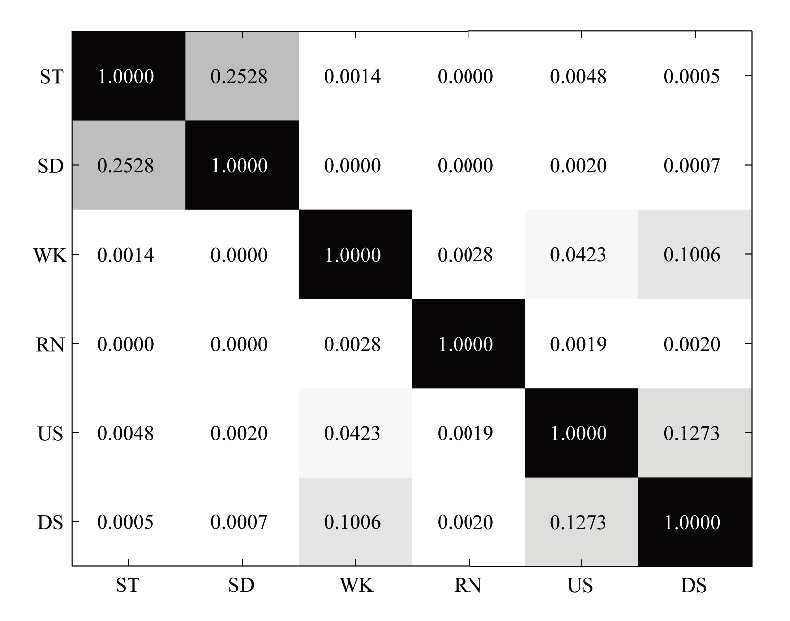
\includegraphics[width=0.6\textwidth]{similarity.eps}
\caption{行为之间的相似度}
\end{figure}
\par 根据相似度行为的分类结果如表格所示,此结果也刚好符合我们正常的思维习惯。
\begin{table}[!htbp]
\centering
\caption{The result of activity grouping}\label{tab:aStrangeTable}
\begin{tabular}{cl}
\toprule
Type& Activity\\
\midrule
\multirow{2}*{Static}
&Sitting(ST)\\
&Standing(SD)\\
\hline
\multirow{3}*{Slow Dynamic}
&Walking(WK)\\
&Ascending Stair(AS)\\
&Descending Stair(DS)\\
\hline
\multirow{1}*{Fast Dynamic}
&Running(RN)\\
\bottomrule
\end{tabular}
\end{table}
\subsection{静态行为分类策略}
\par 对于静态行为,比如坐和站的状态,它们的运动特征几乎没有区别,因此根据加速度等信息很难区分它们。另外,也不能像基于可穿戴传感器的行为识别中使用方向信息进行判断,因为手机并不是相对于人体是固定不变的。为此,在本文中我们提出一种间接的策略区分静态行为,即引入转换行为状态。例如,对于区分坐和站,转换状态,包括坐下和站起等,可以帮助区分两类静止行为。本文中区分静止行为的方法框架如图4所示。
\par 如图4所示,如果前一次第一层分类的识别结果为静态行为且陀螺仪关于角速度的信号模值的最值没有超过之前设定的阈值,则此次保持上次的判决结果。否则,对前一个判决周期内的转换行为利用之前训练的分类器进行分类。根据这一分类器的分类结果,间接推断出静止的行为状态。
\begin{figure}[!htp]
\centering
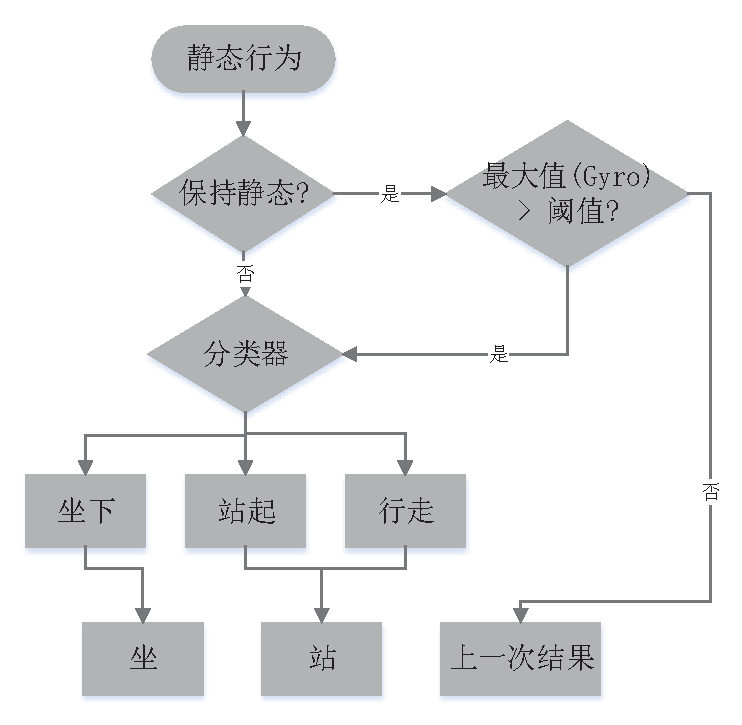
\includegraphics[width=0.6\textwidth]{static_strategy.eps}
\caption{静态行为分类策略流程图}
\end{figure}

\subsection{动态行为分类策略}
\par 对于动态的行为,运动传感器所采集的数据很容易受到位置和方向变化的影响,因为当手机处于人体不同位置时,加速度等信息会表现出不同的信号模式。因此分类器对动态行为的分类很容易受到手机所处位置和方向变化的影响,尤其是对于那些相似行为,即被分在同一组的行为。在本文中,我们提出一种位置辅助分类器的方法可以有效降低位置变化带来的影响。该方法的关键就是对于每一次判定为动态行为时,首先使用之前训练的位置分类器对其分类获取其位置信息。然后再针对不同位置,使用相应位置下所选取的最佳特征集以及所训练的分类器对其进行最终的行为分类。在本文中,在采集数据时智能手机分别被放置在四个不同位置,分别是手中,上衣口袋,裤子口袋,裤子背面口袋。在训练位置分类器时,上衣口袋被定义为上身位置,裤子口袋和裤子背部口袋被定义为下身位置。动态行为分类策略的过程如图5所示。引入位置辅助分类器不但可以有效降低位置变化带来的影响,而且还可以根据不同位置下运动传感器的不同特征选择各自最佳的特征集,进而训练各自最佳的分类器,可以有效改善最终的分类结果。
\begin{figure}[!htp]
 \centering
 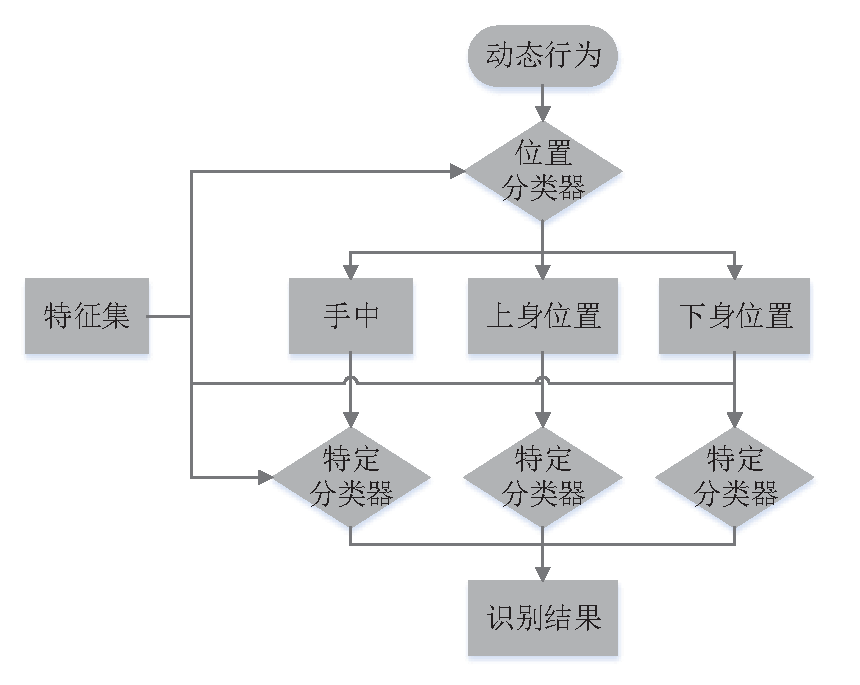
\includegraphics[width=0.8\textwidth]{dynamic_strategy.eps}
 \caption{动态行为分类策略}
\end{figure}


\section{分类实验结果}
\subsection{数据采集实验以及参数设定}
\par 在实验过程中,我们共有6人参与数据集的采集,而我们最初将所有传感器的采样率都设定为$50Hz$。我们所采集的数据集的时间分布如表格所示。所采集的数据会通过滑动窗口的方法对其进行分段,窗口的时间长度为$T=5s$,重叠率为50\%。对于每一个窗口内的数据可以提取我们前面所提到的一系列特征,然后分一个分类器都可以根据特征的信息增益选择最佳的特征集。在实验过程中,我们设定都选择信息增益最高的10个特征。

\begin{table}[!htbp]
\centering
\caption{The data set distribution}\label{tab:aStrangeTable}
\begin{tabular}{|c|c|c|c|c|c|c|}
\hline
\diagbox{Position}{Time(minute)}{Activity} &ST &SD &WK &RN &AS &DS\\
\hline
Hand &12 &12 &30 &30 &30 &30\\
\hline
Coat Pocket &12 &12 &30 &30 &30 &30\\
\hline
Trouser Pocket &12 &12 &30 &30 &30 &30\\
\hline
Rear Pocket &0 &12 &30 &30 &30 &30\\
\hline
\end{tabular}
\end{table}

\par 对于分类器的选择,我们统一都是用随机森林作为默认的分类算法,该算法在\cite{bin2012classification}中,作者已经通过实验验证了其对行为识别的有效性。在计算每一层分类器的分类结果时,我们采用选择其中五个参与者的数据作为训练集,剩余一个参与者的数据作为测试集,然后依次执行六次,计算这六次的平均值。在本文中,结果的评定指标包括正例正确率(True Positive, TP),误报率(False Positiove, FP),准确率(Precision),召回率(Recall),F系数(F-Measure)等。

\subsection{分类结果与分析}
\par 将所有行为分为三组以后,相应数据也合并为有三个类标签的数据,进而训练相应的随机森林分类器。在第一层使用该分类器对数据进行分组,其结果如表格3所示。由于根据之前的分组原则,不同组之间行为的差异很大,所以第一层的识别效果比较好。
%第一层分类结果
    \begin{table}[!ht]
    \centering
    \caption{the results in the first layer}
    \begin{tabular}{cccccc}
    \toprule
    Classes & TP Rate & FP Rate & Precision & Recall & F-Measure \\
    \midrule
    Static & 0.997 & 0.001 & 0.997 & 0.997 & 0.997 \\
    Slow Dynamic & 0.997 & 0.004 & 0.997 & 0.997 & 0.997 \\
    Fast Dynamic & 0.993 & 0.001 & 0.992 & 0.993 & 0.993\\
    \hline
    Weighted Avg. & 0.997 & 0.003 & 0.997 & 0.997 & 0.997\\
    \bottomrule
    \end{tabular}
    \end{table}
%静态行为分类策略结果
\par 对于静态行为,本文仅以坐和站为例, 因此实验过程中采集了坐下、站起以及从静止变为行走等过渡状态下的数据。实验参与者周期性地进行坐下、站起、行走等,周期时间长度设定为15s。在这个过程中陀螺仪所采集的数据如图10所示。

%此处加转换状态下的陀螺仪数据图

\par 传感器数据被分段,时间窗口长度依然为 ,但是不再有重叠。然后从这些时间窗口内的数据中提取相应特征并利用训练数据训练随机森林分类器。最后使用该分类器对过渡行为进行分类,分类结果如表格4所示。而通过过渡态的行为分类,根据我们之前所述的静态行为分类方法即可以间接获取静态的行为状态。

\begin{table}[!ht]
    \centering
    \caption{静态行为分类策略的分类结果}
    \begin{tabular}{cccccc}
    \toprule
    Classes & TP Rate & FP Rate & Precision & Recall & F-Measure \\
    \midrule
    Sit-Stand & 0.9848 & 0.0014 & 0.9924 & 0.9848 & 0.9886\\
    Stand-Sit & 0.9924 & 0.0056 & 0.9704 & 0.9924 & 0.9813\\
    Walking & 0.9966 & 0 & 1.0000 & 0.9966 & 0.9983\\
    \hline
    Weighted Avg & 0.9941 & 0.0011 & 0.9942 & 0.9941 & 0.9941\\
    \bottomrule
    \end{tabular}
 \end{table}

 %动态行为分类策略结果
\par 在实验过程中,我们同样计算了位置分类器的分类准确率,这对于位置辅助的动态行为分类是十分重要的。如表格5所示,位置分类器的分类准确率较高,因此首先进行的位置分类对于行为分类结果的准确率影响并不大,也就表明位置辅助的动态行为识别方法有其重要的意义。

%位置分类器的分类结果
 \begin{table}[!htb]
    \centering
    \caption{动态行为分类策略的分类结果}
    \begin{tabular}{cccccc}
    \toprule
    Classes & TP Rate & FP Rate & Precision & Recall & F-Measure \\
    \midrule
    Hand & 0.9927 & 0.0033 & 0.9937 & 0.9927 & 0.9932\\
    Upper Body & 0.9282 & 0.0163 & 0.9058 & 0.9282 & 0.9169	\\
    Lower Body & 0.9720 & 0.0228 & 0.9782 & 0.9720 & 0.9751	\\
    \hline
    Weighted Avg & 0.9728 & 0.0152 & 0.9730 & 0.9728 & 0.9729\\
    \bottomrule
    \end{tabular}
 \end{table}

\par 最后,我们通过对本文提出的两层多策略的分类框架与之前两篇文献\cite{orientationTransation1},\cite{bisio2014comparison}所提出的方法做比较,对分类结果做出分析。为了与之前两篇文献的实验设定一直,本文的行为集中坐和站合并为一类,成为静止状态(SC)。最后的识别结果分别如表格6,7,8所示。
%分类结果比较
 \begin{table}[htb]
    \centering
    \caption{本文框架的分类结果}
    \begin{tabular}{cccccc}
    \toprule
    Classes & TP Rate & FP Rate & Precision & Recall & F-Measure \\
    \midrule
    SC & 0.9972 & 0.0010 & 0.9976 & 0.9972 & 0.9974 \\
    WK & 0.9974 & 0.0201 & 0.9384 & 0.9974 & 0.9575	\\
    RN & 0.9938 & 0.0013 & 0.9925 & 0.9938 & 0.9934	\\
    AS & 0.8926 & 0.0193 & 0.8737 & 0.8926 & 0.8830 \\
    DS & 0.8654 & 0.0132 & 0.9312 & 0.8654 & 0.8971	\\
    \hline
    Weighted Avg & 0.9570 & 0.0095 & 0.9571 & 0.9570 & 0.9567 \\
    \bottomrule
    \end{tabular}
 \end{table}

 \begin{table}[htb]
    \centering
    \caption{文献的分类结果}
    \begin{tabular}{cccccc}
    \toprule
    Classes & TP Rate & FP Rate & Precision & Recall & F-Measure \\
    \midrule
    SC & 0.9988 & 0 & 1.0000 & 0.9988 & 0.9994 \\
    WK & 0.8894 & 0.0245 & 0.9050 & 0.8894 & 0.8971	\\
    RN & 0.9935 & 0.0003 & 0.9978 & 0.9935 & 0.9957	\\
    AS & 0.7991 & 0.0541 & 0.7934 & 0.7991 & 0.7963 \\
    DS & 0.8517 & 0.0420 & 0.8395 & 0.8517 & 0.8456	\\
    \hline
    Weighted Avg & 0.9039 & 0.0249 & 0.9044 & 0.9039 & 0.9041 \\
    \bottomrule
    \end{tabular}
 \end{table}

  \begin{table}[htb]
    \centering
    \caption{文献的分类结果}
    \begin{tabular}{cccccc}
    \toprule
    Classes & TP Rate & FP Rate & Precision & Recall & F-Measure \\
    \midrule
    SC & 0.9776 & 0.0012 & 0.9965 & 0.9776 & 0.9869 \\
    WK & 0.7714 & 0.0758 & 0.7319 & 0.7714 & 0.7511 \\
    RN & 0.9946 & 0.0011 & 0.9935 & 0.9946 & 0.9941 \\
    AS & 0.7456 & 0.0489 & 0.7894 & 0.7456 & 0.7669 \\
    DS & 0.7342 & 0.0659 & 0.7171 & 0.7342 & 0.7256 \\
    
    Weighted Avg & 0.8455 & 0.0384 & 0.8475 & 0.8455 & 0.8462 \\
    \bottomrule
    \end{tabular}
 \end{table}